%%%%%%%%%%%%%%%%%%%%%%%%%%%%%%%%%%%%%%%%%%%%%%%%%%%
\begin{frame}
  \begin{center}
    {\Large Self Organizing Maps (SOM)}
    
\tiny{(Ref: Deep Learning A-Z -  Kirill Eremenko)}      
  \end{center}
  

\end{frame}

%%%%%%%%%%%%%%%%%%%%%%%%%%%%%%%%%%%%%%%%%%%%%%%%%%%
\begin{frame}[fragile] \frametitle{Introduction}

Unsupervised method invented by Kohonen (also called as Kohonen Maps)


\begin{center}
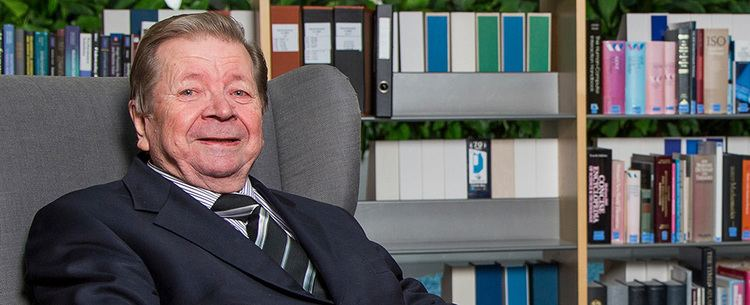
\includegraphics[width=0.8\linewidth,keepaspectratio]{som1}

\tiny{(Ref: https://alchetron.com/Teuvo-Kohonen)}
\end{center}

\end{frame}

%%%%%%%%%%%%%%%%%%%%%%%%%%%%%%%%%%%%%%%%%%%%%%%%%%%
\begin{frame}[fragile] \frametitle{Introduction}
Useful in reducing dimensions.

\begin{center}
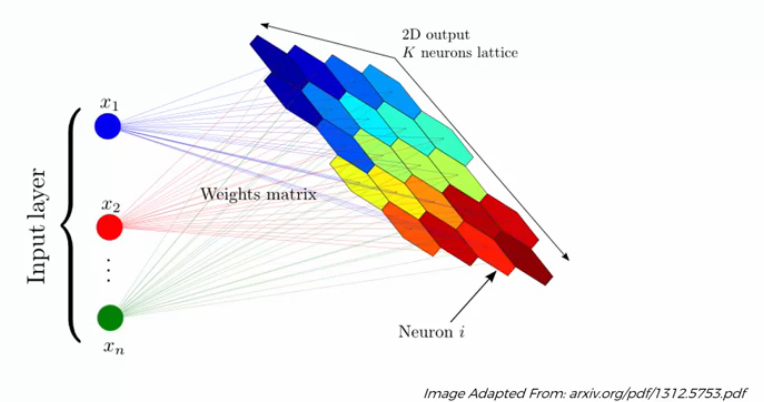
\includegraphics[width=\linewidth,keepaspectratio]{som2}
\end{center}

\end{frame}


%%%%%%%%%%%%%%%%%%%%%%%%%%%%%%%%%%%%%%%%%%%%%%%%%%%
\begin{frame}[fragile] \frametitle{How SOM works?}
Actual picture of a SOM

\begin{center}
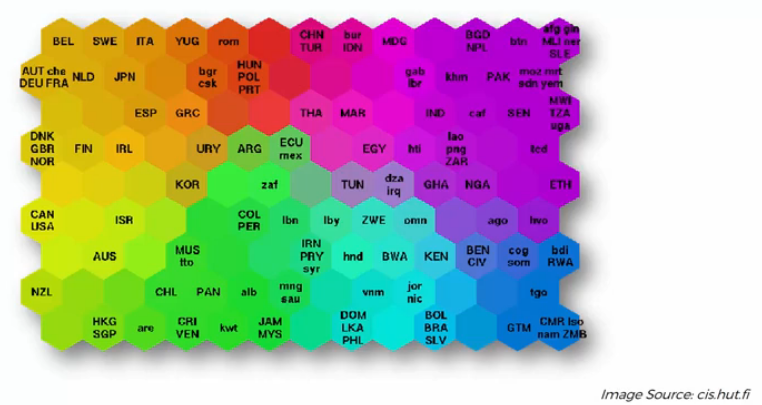
\includegraphics[width=0.8\linewidth,keepaspectratio]{som3}
\end{center}

Counties of the world, clustered them based on 39 indiciators such a nuitrition, education, et.c 39 were reduced to 2D for visualization.
Left are least poverty and right most poverty.
\end{frame}

%%%%%%%%%%%%%%%%%%%%%%%%%%%%%%%%%%%%%%%%%%%%%%%%%%%
\begin{frame}[fragile] \frametitle{How SOM works?}
Clustering based on similarities between countries. We take those colors and put them in normal geo map.

\begin{center}
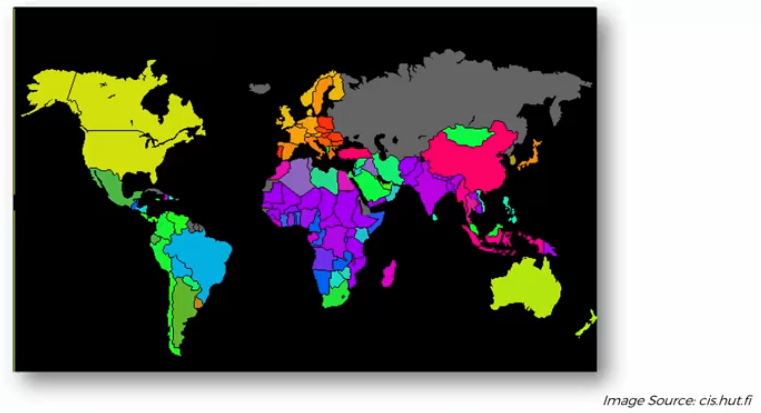
\includegraphics[width=0.8\linewidth,keepaspectratio]{som4}
\end{center}

Clustring (thus coloring) done by SOM appears to be matching with what we can guess here.
\end{frame}

%%%%%%%%%%%%%%%%%%%%%%%%%%%%%%%%%%%%%%%%%%%%%%%%%%%
\begin{frame}[fragile] \frametitle{How SOM works?}
Total process:
\begin{itemize}
\item Getting data from World organizations. 39 features.
\item Apply SOM to form clusters and make it 2D
\item Pick the colors from SOM and apply them on Geo map.
\end{itemize}

\begin{center}
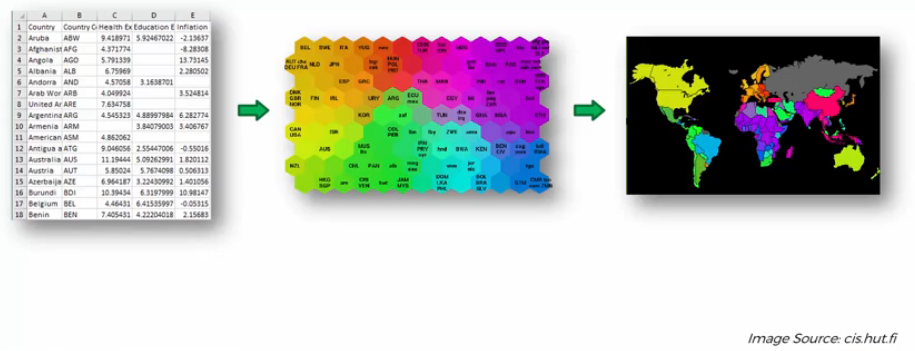
\includegraphics[width=0.8\linewidth,keepaspectratio]{som5}
\end{center}

Clustring (thus coloring) done by SOM appears to be matching with what we can guess here.
\end{frame}


%%%%%%%%%%%%%%%%%%%%%%%%%%%%%%%%%%%%%%%%%%%%%%%%%%%
\begin{frame}[fragile] \frametitle{How SOM works?}
Simple example: 3 input features (many rows) and 9 values in output.

\begin{center}
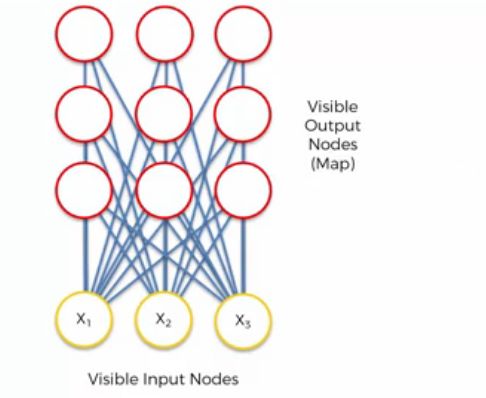
\includegraphics[width=0.6\linewidth,keepaspectratio]{som6}
\end{center}
\end{frame}

%%%%%%%%%%%%%%%%%%%%%%%%%%%%%%%%%%%%%%%%%%%%%%%%%%%
\begin{frame}[fragile] \frametitle{How SOM works?}
Let's look at equivalent structure

\begin{center}
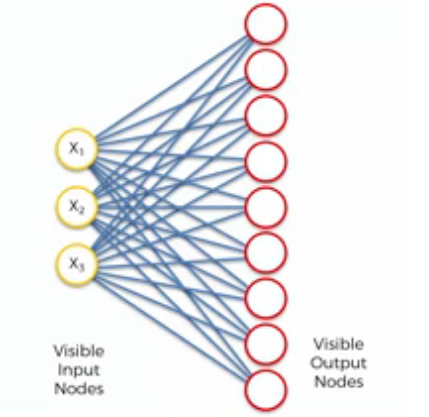
\includegraphics[width=0.6\linewidth,keepaspectratio]{som7}
\end{center}
\end{frame}

%%%%%%%%%%%%%%%%%%%%%%%%%%%%%%%%%%%%%%%%%%%%%%%%%%%
\begin{frame}[fragile] \frametitle{How SOM works?}
\begin{itemize}
\item Let's look at subset edges with weights (indices output id, input node id)
\item No activations, no wighted sum.
\item Its like, Output Node 1 is represented by coordinates x1,x2,x3.
\end{itemize}
\begin{center}
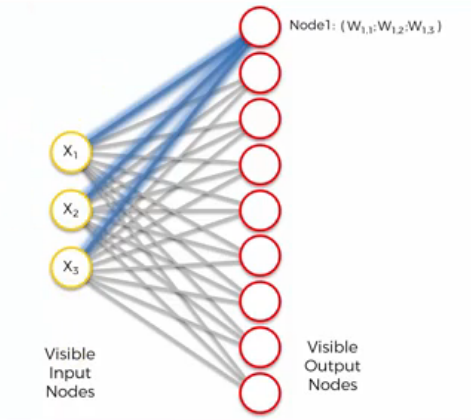
\includegraphics[width=0.5\linewidth,keepaspectratio]{som8}
\end{center}
\end{frame}

%%%%%%%%%%%%%%%%%%%%%%%%%%%%%%%%%%%%%%%%%%%%%%%%%%%
\begin{frame}[fragile] \frametitle{How SOM works?}
\begin{itemize}
\item Similarly other output nodes are represented by input features as coordinates.
\item At starts weights have random values. So output nodes are random points in n\_features\_dimensional space.
\end{itemize}
\begin{center}
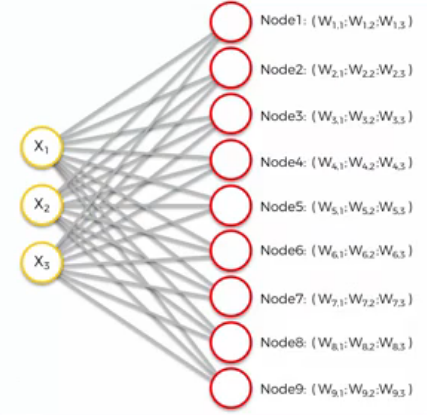
\includegraphics[width=0.5\linewidth,keepaspectratio]{som9}
\end{center}
\end{frame}

%%%%%%%%%%%%%%%%%%%%%%%%%%%%%%%%%%%%%%%%%%%%%%%%%%%
\begin{frame}[fragile] \frametitle{How SOM works?}
\begin{itemize}
\item Go through rows one by one and see which nodes match best
\item Its based on distance between xs and ws for each node.
\end{itemize}
\begin{center}
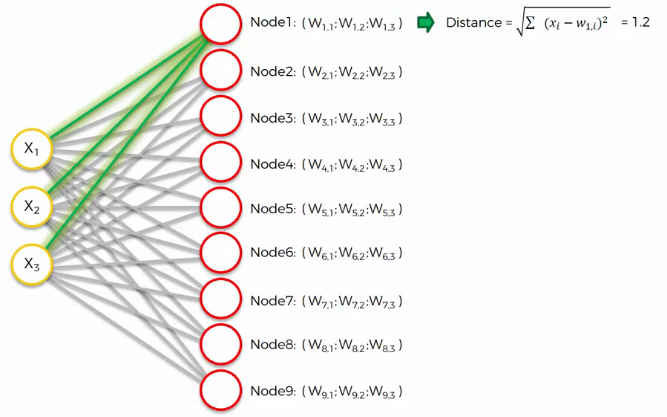
\includegraphics[width=0.8\linewidth,keepaspectratio]{som10}
\end{center}
\end{frame}

%%%%%%%%%%%%%%%%%%%%%%%%%%%%%%%%%%%%%%%%%%%%%%%%%%%
\begin{frame}[fragile] \frametitle{How SOM works?}
The least distance for row 1 is node 3
\begin{center}
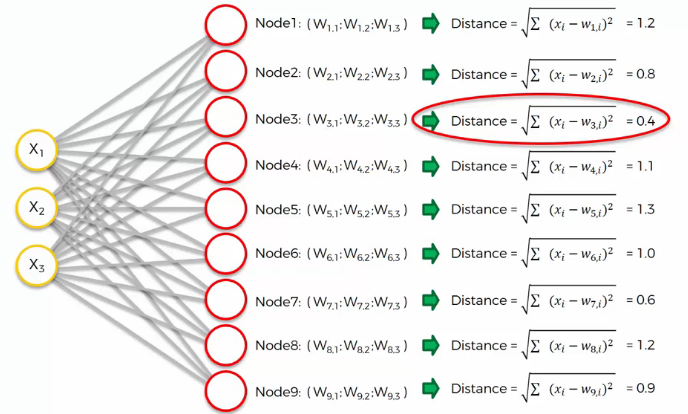
\includegraphics[width=0.8\linewidth,keepaspectratio]{som11}
\end{center}
\end{frame}

%%%%%%%%%%%%%%%%%%%%%%%%%%%%%%%%%%%%%%%%%%%%%%%%%%%
\begin{frame}[fragile] \frametitle{How SOM works?}
\begin{itemize}
\item Weights are updated for best node so that it becomes MORE CLOSER
\item Once all rows are done, the weights of the nodes get MOST close to the underlying data.
\item It Self Organizes onto your input data (thus SOM)
\end{itemize}
\begin{center}
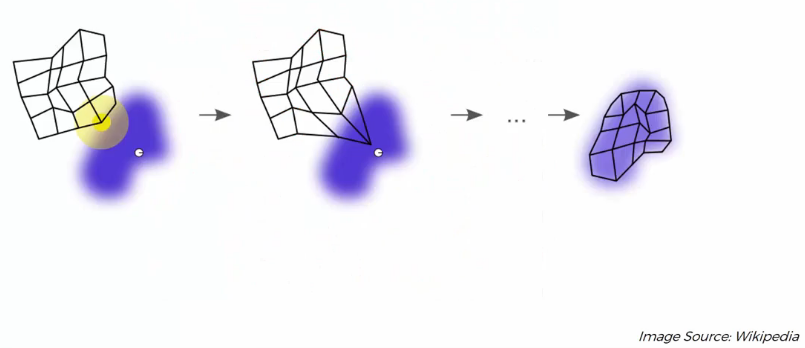
\includegraphics[width=0.8\linewidth,keepaspectratio]{som12}
\end{center}
\end{frame}

%%%%%%%%%%%%%%%%%%%%%%%%%%%%%%%%%%%%%%%%%%%%%%%%%%%
\begin{frame}[fragile] \frametitle{How SOM works?}
\begin{itemize}
\item As one node gets dragged, even some of the nearby points get dragged proportionately.
\item So, nodes inside influence zone, their weights get updated.
\item Closer to best node, more update happens
\end{itemize}
\begin{center}
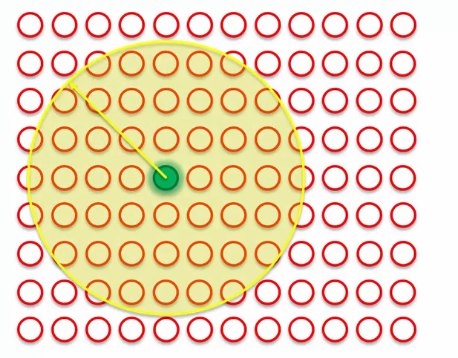
\includegraphics[width=0.8\linewidth,keepaspectratio]{som13}
\end{center}
\end{frame}

%%%%%%%%%%%%%%%%%%%%%%%%%%%%%%%%%%%%%%%%%%%%%%%%%%%
\begin{frame}[fragile] \frametitle{How SOM works?}
\begin{itemize}
\item As one node gets dragged, even some of the nearby points get dragged proportionately.
\item So, nodes inside influence zone, their weights get updated.
\item Closer to best node, more update happens
\end{itemize}
\begin{center}
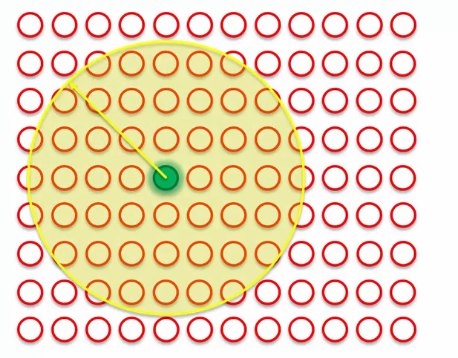
\includegraphics[width=0.8\linewidth,keepaspectratio]{som13}
\end{center}
\end{frame}

%%%%%%%%%%%%%%%%%%%%%%%%%%%%%%%%%%%%%%%%%%%%%%%%%%%
\begin{frame}[fragile] \frametitle{How SOM works?}
\begin{itemize}
\item If there are multiple best nodes (or specified K), their influence zones overlap and thus proportionalty the resultnatnt movement direction gets chosen (vector sum)
\item In each iteration, the influence zones reduce.
\item Once the data maps well, no more movement is possible.
\end{itemize}
\begin{center}
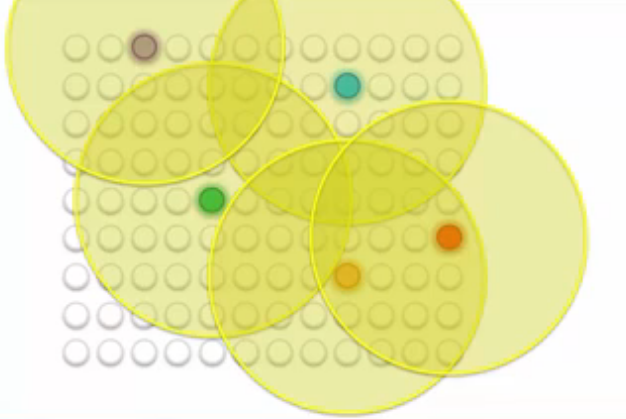
\includegraphics[width=0.5\linewidth,keepaspectratio]{som14}
\end{center}
\end{frame}


%%%%%%%%%%%%%%%%%%%%%%%%%%%%%%%%%%%%%%%%%%%%%%%%%%%
\begin{frame}[fragile] \frametitle{How SOM works?}
\begin{itemize}
\item Naturally groups get formed based on the distance.
\item Meaning set of rows gets clusterd, almost lke K-Means.
\end{itemize}
\begin{center}
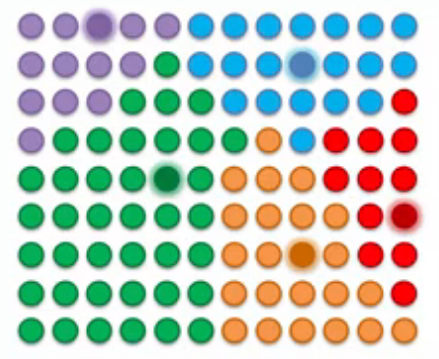
\includegraphics[width=0.5\linewidth,keepaspectratio]{som15}
\end{center}
\end{frame}

%%%%%%%%%%%%%%%%%%%%%%%%%%%%%%%%%%%%%%%%%%%%%%%%%%%
\begin{frame}[fragile] \frametitle{Note}
\begin{itemize}
\item SOMs retain topology of the input data
\item SOMs reveal correlations that are not easily idenified
\item SOMs classify data without supervision
\item No Labels so NO Backpropogation.
\end{itemize}

\end{frame}